\documentclass{beamer}
\usepackage{tikz}
\usetikzlibrary{arrows,shapes}
\tikzstyle{vertex}=[circle,fill=black!25,minimum size=10pt,inner sep=0pt]
\tikzstyle{blue vertex}=[circle,fill=blue!100,minimum size=10pt,inner sep=0pt]
\tikzstyle{red vertex}=[circle,fill=red!100,minimum size=10pt,inner sep=0pt]
%\tikzstyle{label}=[thin, draw=black, align=center,minimum width=0.5cm, minimum height=0.5cm,fill=white]
\tikzstyle{edge} = [draw,thick,-]
\tikzstyle{red edge} = [draw, line width=5pt,-,red!50]
\tikzstyle{black edge} = [draw, line width=5pt,-,black!20]
\tikzstyle{weight} = [font=\smaller]


\usepackage{amssymb,amsmath}
\usepackage{graphicx}
\usepackage{url}
\usepackage{color}
\usepackage{relsize}		% For \smaller
\usepackage{url}			% For \url
\usepackage{epstopdf}	% Included EPS files automatically converted to PDF to include with pdflatex
\usepackage{pagenote}[continuous,page]

%For MindMaps
% \usepackage{tikz}%
% \usetikzlibrary{mindmap,trees,arrows}%

%%% Color Definitions %%%%%%%%%%%%%%%%%%%%%%%%%%%%%%%%%%%%%%%%%%%%%%%%%%%%%%%%%
%\definecolor{bordercol}{RGB}{40,40,40}
%\definecolor{headercol1}{RGB}{186,215,230}
%\definecolor{headercol2}{RGB}{80,80,80}
%\definecolor{headerfontcol}{RGB}{0,0,0}
%\definecolor{boxcolor}{RGB}{186,215,230}

%%% Save space in lists. Use this after the opening of the list %%%%%%%%%%%%%%%%
%\newcommand{\compresslist}{
%	\setlength{\itemsep}{1pt}
%	\setlength{\parskip}{0pt}
%	\setlength{\parsep}{0pt}
%}

%\setbeameroption{show notes on top}

% You should run 'pdflatex' TWICE, because of TOC issues.

% Rename this file.  A common temptation for first-time slide makers
% is to name it something like ``my_talk.tex'' or
% ``john_doe_talk.tex'' or even ``discrete_math_seminar_talk.tex''.
% You really won't like any of these titles the second time you give a
% talk.  Try naming your tex file something more descriptive, like
% ``riemann_hypothesis_short_proof_talk.tex''.  Even better (in case
% you recycle 99% of a talk, but still want to change a little, and
% retain copies of each), how about
% ``riemann_hypothesis_short_proof_MIT-Colloquium.2000-01-01.tex''?

\mode<presentation>
{
  % A tip: pick a theme you like first, and THEN modify the color theme, and then add math content.
  % Warsaw is the theme selected by default in Beamer's installation sample files.

  %%%%%%%%%%%%%%%%%%%%%%%%%%%% THEME
  %\usetheme{Madrid}		% No subsection
  \usetheme{AnnArbor}  % Subsection on top, no color


  %\usetheme{Antibes}
  %\usetheme{Bergen}
  %\usetheme{Berkeley}		% bem bacana - menu esquerdo
  %\usetheme{Berlin}
  %\usetheme{Boadilla}
  %\usetheme{boxes}
  %\usetheme{CambridgeUS}		% bem bacana - menu superior
  %\usetheme{Copenhagen}
  %\usetheme{Darmstadt}
  %\usetheme{default}
  %\usetheme{Dresden}
  %\usetheme{Frankfurt}
  %\usetheme{Goettingen}
  %\usetheme{Hannover}		% bem bacana - menu esquerdo
  %\usetheme{Ilmenau}
  %\usetheme{JuanLesPins}
  %\usetheme{Luebeck}
  %\usetheme{Malmoe}
  %\usetheme{Marburg}		% bem bacana - menu direito
  %\usetheme{Montpellier}
  %\usetheme{PaloAlto}		% bem bacana - menu esquerdo
  %\usetheme{Pittsburgh}
  %\usetheme{Rochester}		%bacana
  %\usetheme{Singapore}
  %\usetheme{Szeged}
  %\usetheme{Warsaw}

  %%%%%%%%%%%%%%%%%%%%%%%%%%%% COLOR THEME
  %\usecolortheme{default}		% branco, azul clarinho
  \usecolortheme{crane}		% Very yellow (ok)

  %\usecolortheme{albatross}		% azul escuro, massa
  %\usecolortheme{beetle}		% cinza, menu azul
  %\usecolortheme{dolphin}		% azul e branco, legal
  %\usecolortheme{dove}			% cinza e branco, feio
  %\usecolortheme{fly}			% todo cinza, horrível
  %\usecolortheme{lily}			% parece o default
  %\usecolortheme{orchid}		% azul e branco, ok
  %\usecolortheme{rose}			% branco e violeta-claro, bonito
  %\usecolortheme{seagull}		% cinza, feio
  %\usecolortheme{seahorse}		% nhé, meio feio
  %\usecolortheme{sidebartab}		% Azul, branco, destaque na tab, interessante
  %\usecolortheme{structure}		% bichado
  %\usecolortheme{whale}		% Azul e branco, bem bonito

  %%%%%%%%%%%%%%%%%%%%%%%%%%%% OUTER THEME
  \useoutertheme{default}
  %\useoutertheme{infolines}
  %\useoutertheme{miniframes}
  %\useoutertheme{shadow}
  %\useoutertheme{sidebar}
  %\useoutertheme{smoothbars}
  %\useoutertheme{smoothtree}
  %\useoutertheme{split}
  %\useoutertheme{tree}

  %%%%%%%%%%%%%%%%%%%%%%%%%%%% INNER THEME
  \useinnertheme{circles}
  %\useinnertheme{default}
  %\useinnertheme{inmargin}
  %\useinnertheme{rectangles}
  %\useinnertheme{rounded}

  %%%%%%%%%%%%%%%%%%%%%%%%%%%%%%%%%%%

  \setbeamercovered{invisible} % or whatever (possibly just delete it)
  % To change behavior of \uncover from graying out to totally
  % invisible, can change \setbeamercovered to invisible instead of
  % transparent. apparently there are also 'dynamic' modes that make
  % the amount of graying depend on how long it'll take until the
  % thing is uncovered.

}


% Get rid of nav bar
\beamertemplatenavigationsymbolsempty

% Use short top
%\usepackage[headheight=12pt,footheight=12pt]{beamerthemeboxes}
%\addheadboxtemplate{\color{black}}{
%\hskip0.5cm
%\color{white}
%\insertshortauthor \ \ \ \
%\insertframenumber \ \ \ \ \ \ \
%\insertsection \ \ \ \ \ \ \ \ \ \ \ \ \ \ \ \ \  \insertsubsection
%\hskip0.5cm}
%\addheadboxtemplate{\color{black}}{
%\color{white}
%\ \ \ \
%\insertsection
%}
%\addheadboxtemplate{\color{black}}{
%\color{white}
%\ \ \ \
%\insertsubsection
%}

% Insert frame number at bottom of the page.
% \usefoottemplate{\hfil\tiny{\color{black!90}\insertframenumber}}

%% makes the ppagenote command for figure references at the end.

\usepackage[english]{babel}
%qq\usepackage[latin1]{inputenc}
\usepackage{CJKutf8}
\usepackage{subfigure}

\usepackage{times}
\usepackage[T1]{fontenc}

\makepagenote
\renewcommand{\notenumintext}[1]{}
\newcommand{\ppagenote}[1]{\pagenote[Page \insertframenumber]{#1}}

\title[Programming Challenges]{GB20602 - Programming Challenges}
\author[Claus Aranha]{Claus Aranha\\{\footnotesize caranha@cs.tsukuba.ac.jp}}
\institute[U. Tsukuba]{University of Tsukuba, Department of Computer Sciences}


\subtitle[Week 9: Geometry]{Week 9 - Computational Geometry}
\date[2020/6/23]{2020/6/23\\{\smaller(last updated: \today)}}

\begin{document}
\begin{CJK}{UTF8}{ipxm}

\begin{frame}
\maketitle
\vfill

\hfill Version 2020.1
\end{frame}


\section{Introduction}

\begin{frame}
  \frametitle{Computational Geometry}
  \framesubtitle{What is it?}

  {\small

    \structure{Computational Geometry} problems involve answering
    questions about \structure{lines, points and angles}. Some example
    questions:

    \bigskip

    \begin{block}{}
    \only<1>{Given $N$ points $(s_1, s_2, s_3, \ldots, s_N)$, what is
      the area of the poligon that covers all the points?}

    \only<2>{Given $N$ rectangles, $x_1,y_1,w_1,h_1; \ldots; x_N, y_N,
      w_N, h_N$, what is the length of lines needed to connect them?}

    \only<3>{Given a polygon, and $N$ points, what is the line
      that divides the polygon in equal areas, so that the same
      number of points are in each area?}
    \end{block}

    \begin{center}
      \includegraphics<1>[width=0.8\textwidth]{img/sampleproblem_1.png}
      \includegraphics<2>[width=0.6\textwidth]{img/sampleproblem_2.png}
      \includegraphics<3>[width=0.4\textwidth]{img/sampleproblem_3.png}
    \end{center}

  }
\end{frame}

\begin{frame}
  \frametitle{Computational Geometry}
  \framesubtitle{The good and the bad}

  \begin{itemize}
  \item \structure{Good}: Geometry problems are fun
  \item \structure{Good}: You have to draw pretty pictures
  \item \structure{Good}: Mostly algorithms from high school
  \item \structure{Good}: Code is highly re-usable

    \bigskip

  \item \alert{Bad}: You have to write a lot of code (in the beginning!)
  \item \alert{Bad}: Very easy to get WE...
  \end{itemize}
\end{frame}


\begin{frame}
  \frametitle{Easy Mistakes in Geometry Problems}

  {\small
    \begin{block}{Problem 1 -- Special Cases}
      \begin{itemize}
      \item Multiple points in the same place;
      \item Collinear points;
      \item Vertical lines;
      \item Parallel Lines;
      \item Intersection at end of segment;
      \item etc;
      \end{itemize}
    \end{block}

    \begin{block}{Problem 2 -- Precision Errors}
      \begin{itemize}
      \item Functions require many multiplications and divisions;
      \item Easy to propagate floating point errors;
      \end{itemize}
    \end{block}
  }
\end{frame}


\begin{frame}[fragile]
  \frametitle{Easy Mistakes in Geometry Problems}

  {\smaller

    \begin{block}{Dealing Special Cases}
      \begin{itemize}
      \item Make sure to add special cases to your
        library functions;
      \end{itemize}
    \end{block}

    \begin{block}{Solving Precision Errors}
      \begin{itemize}
      \item If possible, convert all values to integers
      \item Use an EPSILON constant for comparisons:

\begin{verbatim}
if (float.1 == float.2) then            // NO
if (fabs(float.1 - float.2) < EPS) then // YES!
\end{verbatim}

      \end{itemize}
    \end{block}
  }
\end{frame}

\begin{frame}
  \frametitle{Class Outline}
  \begin{itemize}
  \item Example Problems;
  \item Basic Geometric Functions;
  \item Circles;
  \item Triangles;
  \item Polygons;
  \end{itemize}
\end{frame}



\section{Basic Functions}
\begin{frame}
  \centering
  {\bf Part II -- Points and Lines}
\end{frame}

\subsection{Points}
\begin{frame}[fragile]{Representing a point as a structure}
    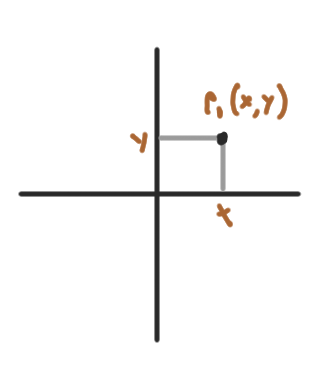
\includegraphics[width=.15\textwidth]{../img/geom2}
    \begin{exampleblock}{}
\begin{verbatim}
struct point_i { int x, y;  // integer coordinates
  point_i() { x = y = 0; }
  point_i(int _x, int _y) : x(_x), y(_y) {}};

struct point { double x, y; // double coordinates
  point() { x = y = 0.0;}
  point(double _x, double _y) : x(_x), y(_y) {}};
\end{verbatim}
    \end{exampleblock}
\end{frame}

\begin{frame}[fragile]{Overloading Point Operators}

    \begin{exampleblock}{}
      {\smaller
\begin{verbatim}
struct point { double x, y;
   point() { x = y = 0.0;
   point(double _x, double _y) : x(_x), y(_y) {}

   bool operator < (point other) const {           // Overloading "<"
      if (fabs(x - other.x) > EPS)
         return x < other.x;
      return y < other.y; }
   bool operator == (point other) const {          // Overloading "=="
      return (fabs(x - other.x) < EPS &&
             (fabs(y - other.y) < EPS)); }
   }

point a = point(1,2); point b = point(3,4);

if (!(a == b)) printf("Different\n");
\end{verbatim}}
    \end{exampleblock}
\end{frame}

\begin{frame}[fragile]{Point Distance}
    \begin{exampleblock}{}
{\smaller
\begin{verbatim}
// Euclidean Distance: "normal" distance
#define hypot(dx,dy) sqrt(dx*dx + dy*dy)
double dist(point p1, point p2) { return hypot(p1.x - p2.x, p1.y - p2.y); }

// Taxicab Distance / Manhattan Distance : Distance on a grid
double taxicab(point p1, point p2) { return fabs(p1.x-p2.x) + fabs(p1.y-p2.y); }
\end{verbatim}}
    \end{exampleblock}

    \begin{center}
      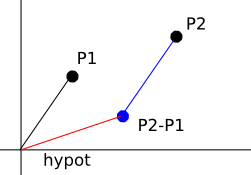
\includegraphics[width=0.4\textwidth]{../img/geom1}
    \end{center}
\end{frame}

\begin{frame}[fragile]{Point Rotation}

  {\smaller

    \begin{exampleblock}{}
\begin{verbatim}
#define PI           3.14159265358979323846  // Pi constant
double PI = 2 * acos(0.0)                    // Better Pi
#define DEG_to_RAD(X) (X*PI)/180.0           // Don't confuse DEG and RAD

// suppose angle t is in degrees (0--360)
point rotate(point p, double t) {
   double rad = DEG_to_RAD(t);
   return point(p.x * cos(rad) - p.y * sin(rad),
                p.x * sin(rad) + p.y * cos(rad));}
\end{verbatim}
    \end{exampleblock}
    \begin{center}
      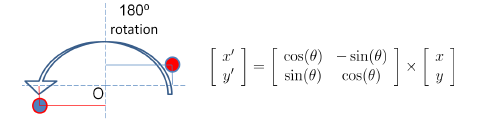
\includegraphics[width=0.8\textwidth]{../img/rotation_halim}
      \ppagenote{Rotation Image from "Competitive Programming 3", Steven Halim}
    \end{center}
}
    {\bf Quiz:} How do you rotate a point around $x_1, y_1$?
\end{frame}

\subsection{Lines}

\begin{frame}[fragile]
  \frametitle{Data Structure for a Line}
  \begin{itemize}
  \item \structure{$ax + by + c = 0$}\hfill (a,b,c) -- useful for most cases
  \item \structure{$y = mx + c$}\hfill (m,c) -- useful for angle manipulation
  \item \structure{$x_0,y_0,x_1,y_1$}\hfill ($p_1, p_2$) -- harder to use, but common input
  \end{itemize}

{\smaller
  \begin{exampleblock}{How to convert from two points to a line}
\begin{verbatim}
struct line { double a,b,c; };

void pointsToLine(point p1, point p2, line &l) {
   if (fabs(p1.x - p2.x) < EPS {
      l.a = 1.0; l.b = 0.0; l.c = -p1.x; }
   else {
      l.a = -(double) (p1.y - p2.y)/(p1.x - p2.x);
      l.b = 1.0; l.c = -(double) (l.a*p1.x) - p1.y;}
}
\end{verbatim}
  \end{exampleblock}
  }
\end{frame}

\begin{frame}[fragile]
  \frametitle{Line Equality}
    \begin{columns}
      \column{0.6\textwidth}
      \begin{itemize}
      \item We define a line as $a,b,c \to (ax+by=c)$

      \item Two lines are parallel if their coefficients $(a, b)$ are the same;\medskip

      \item Two lines are identical if all coefficients $(a,b,c)$ are the same;
      \end{itemize}
      \column{0.4\textwidth}
      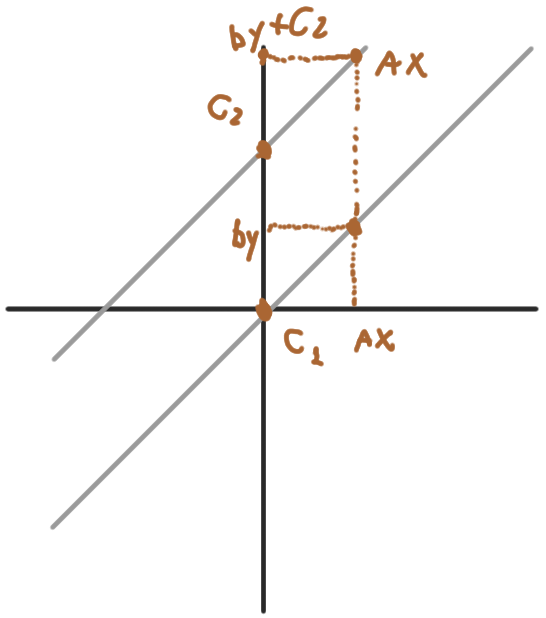
\includegraphics[width=.6\textwidth]{../img/geom3}
    \end{columns}
  \begin{exampleblock}{}
\begin{verbatim}
bool areParallel(line l1, line l2) {
   return (fabs(l1.a-l2.a) < EPS) && (fabs(l1.b-l2.b) < EPS); }

bool areSame(line l1, line l2) {
   return areParallel(l1,l2) && (fabs(l1.c - l2.c) < EPS); }
\end{verbatim}
  \end{exampleblock}
\end{frame}

\begin{frame}[fragile]
  \frametitle{Line Intersection}
    The intersection point $x_I, y_I$ can be found by solving:
    \begin{eqnarray*}
      a_1x_I+b_1y_I+c_1 = 0\\a_2x_I+b_2y_I+c_2 = 0
    \end{eqnarray*}
    Remember that when we create a line $i$, we set $b_i=0$ or $b_i=1$

    {\smaller
    \begin{exampleblock}{}
\begin{verbatim}
bool areIntersect(line l1, line l2, point &p) {
   if (areParallel(l1,l2)) return False;

   p.x = (l2.b * l1.c - l1.b * l2.c) /
         (l2.a * l1.b - l1.a * l2.b);

   // Test for vertical case:
   if (fabs(l1.b) > EPS)     p.y = -(l1.a * p.x + l1.c);
   else                      p.y = -(l2.a * p.x + l2.c);
   return True;
}
\end{verbatim}
    \end{exampleblock}

  }
\end{frame}

\subsection{Segments}
\begin{frame}[fragile]
  \frametitle{Segments and Vectors}
    \begin{columns}
      \column{0.8\textwidth}
      \begin{itemize}
        \item A {\bf line segment} is a line with two endpoints $(p_1, p_2)$;
        \item A {\bf Vector} is a line segment with a direction;
        \begin{itemize}
          \item Usually represented as "direction" and "magnitude";
          \item Direction is a point with distance 1 from $(0,0)$
          \item Magnitude is a multiplier to the size of the vector;
          \item Represent movement, translation, speed, etc;
        \end{itemize}
      \end{itemize}
      \column{0.2\textwidth}
      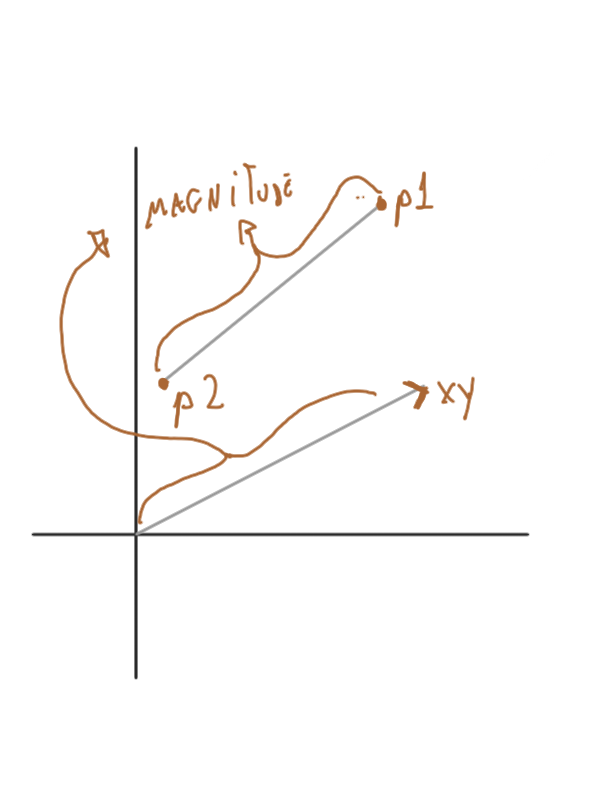
\includegraphics[width=.9\textwidth]{../img/geom4}
    \end{columns}

{\smaller
    \begin{exampleblock}{}
\begin{verbatim}
struct vec { double x, y;
    vec(double _x, double _y) : x(_x), y(_y) {} };

vec toVec(point a, point b) {
    return vec(b.x - a.x, b.y - a.y); }
vec scale(vec v, double s) {
    return vec(v.x * s, v.y * s); }
point translate(point p, vec v) {
    return point(p.x + v.x , p.y + v.y); }
\end{verbatim}
    \end{exampleblock}
  }
\end{frame}

\begin{frame}
  \frametitle{Distance between point and line, point and segment}
  \begin{block}{}
    For a point $p$ and a line $l$ (represented by $\overline{ab}$), the distance between both is given by the segment $pc$, where $c$ is the projection of $p$ in $l$.

    {\smaller
    \begin{columns}[T]
      \column{.5\textwidth}
      Calculating $c$:
      \begin{itemize}
        \item calculate scalar proj. $u$ of $\vec{ap}$ in $l$.
        \item change magnitude of $\vec{ab}$ to $u$ to obtain $\vec{ac}$.
        \item calculate distance between $p$ and $c$.
      \end{itemize}
      \column{.5\textwidth}
      Distance between $p$ and $\overline{ab}$:
      \begin{itemize}
        \item calculate scalar proj. $u$ of $\vec{ap}$ in $l$.
        \item if $u < 0$ or $u > |\vec{ab}|$, then the distance is $\min(d(a,p),d(b,p))$.
        \item else, calculate $\vec{ac}$ and calculate distance $d(p,c)$.
      \end{itemize}
    \end{columns}}
  \end{block}

  \begin{center}
    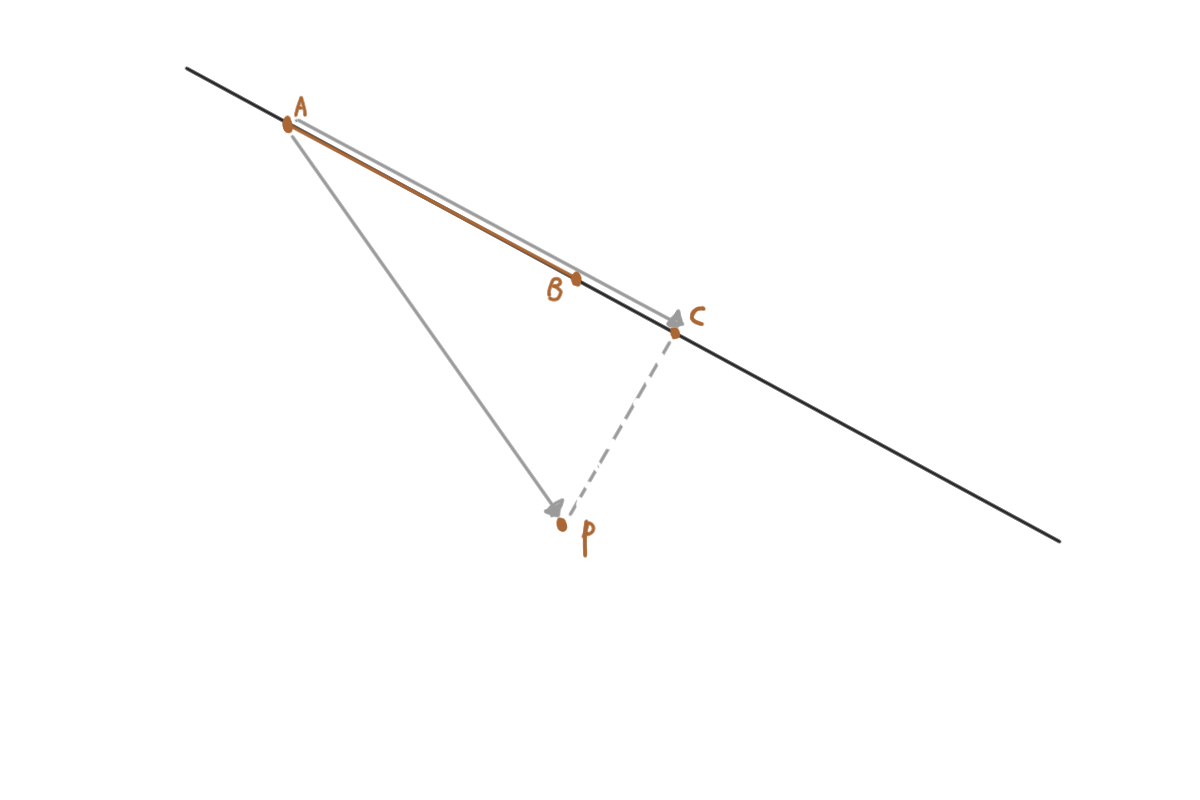
\includegraphics[width=0.5\textwidth]{../img/geom5}
  \end{center}
\end{frame}

\begin{frame}[fragile]
  \frametitle{CODE: Distance between point and line}

  {\smaller
  \begin{exampleblock}{}
\begin{verbatim}
double dot(vec a, vec b) { return (a.x * b.x + a.y * b.y); } // dot product
double norm_sq(vec v) { return v.x * v.x + v.y * v.y; } // norm squared

// Given points a,b,p, calculate distance from p to line ab.
double distToLine(point p, point a, point b, point &c) {
  // point c: c = a + u * |ab|
  vec ap = toVec(a, p), ab = toVec(a, b);

  // dot product calculates size of ap in ab
  // norm square will calculate the scale to ab
  double u = dot(ap, ab) / norm_sq(ab);

  // translate a by u to find point c.
  c = translate(a, scale(ab, u));
  return dist(p, c);
}
\end{verbatim}
  \end{exampleblock}

}
\end{frame}

\begin{frame}[fragile]
  \frametitle{CODE: Distance between point and segment}
  Same as before, but first we test if $c$ is inside $\overline{ab}$.

  {\smaller
    \begin{exampleblock}{}
\begin{verbatim}
double distToSegment(point p, point a, point b, point &c) {
  // next two lines is exact same as last slide
  vec ap = toVec(a, p), ab = toVec(a, b);
  double u = dot(ap, ab) / norm_sq(ab);

  // test if the magnitude $u$ is bigger or smaller than ab.
  if (u < 0.0) { c = point(a.x, a.y); // closer to a
                 return dist(p, a); }
  if (u > 1.0) { c = point(b.x, b.y); // closer to b
                 return dist(p, b); }

  // c is inside AB, same as last slide
  c = translate(a, scale(ab, u));
  return dist(p,c);
}
\end{verbatim}
    \end{exampleblock}
  }
\end{frame}

\begin{frame}[fragile]{Angle between segments}

Given three points, $a$, $b$ and $o$, we can calculate
the angle between $\overline{oa}$ and $\overline{ob}$ using the dot product.\medskip

Given that: $oa\cdot ob = |oa|\times|ob|\times\cos(\theta)$, we have $\theta = \arccos(\frac{oa\cdot ob}{|oa|\times|ob|})$\bigskip

{\smaller

\begin{exampleblock}{}
\begin{verbatim}
#import <cmath>

// angle in radians (0..2*PI)
double angle(point a, point o, point b) {
  vec oa = toVector(o, a), ob = toVector(o, b);
  return acos(dot(oa, ob) / sqrt(norm_sq(oa) * norm_sq(ob)));
}
\end{verbatim}
\end{exampleblock}}
\end{frame}

\begin{frame}[fragile]{Left, Right and Collinear Points}

  Given a line defined by points $p$ and $q$, we are interested in knowing if point $r$ is on the left/right side of the line, or if the three ponts are collinear.\bigskip

  Let $\vec{pq}$ and $\vec{pr}$ be two vectors, the {\bf cross product} $\vec{pq} \times \vec{pr}$ is a vector that is perpendicular to both vectors. The  magnitude of the cross product is positive / zero / negative if $p \to q \to r$ is left turn / collinear / right turn.

  {\smaller
  \begin{exampleblock}{}
  \begin{verbatim}
  double cross(vec a, vec b) { return a.x * b.y - a.y * b.x; }

  bool ccw(point p, point q, point r) {
    return cross(toVec(p, q), toVec(p, r)) > 0; }

  collinear(point p, point q, point r) {
    return fabs(cross(toVec(p, q), toVec(p, r))) < EPS;
  \end{verbatim}
  \end{exampleblock}
  }
\end{frame}

\section{Circles and Triangles}
\begin{frame}
  \centering
  {\bf Part III: Circles and Triangles}
\end{frame}

\begin{frame}[fragile]
  \frametitle{Circles}
  \begin{itemize}
  \item A circle is stored as its center point $c$, and its radius $r$.\medskip

  \item The circle contains all points $(x,y)$ where $(x-a)^2+(y-b)^2 \leq r^2$\medskip

  \item No square root, so less chance of floating point errors.
  \end{itemize}\bigskip

  \begin{exampleblock}{Test if Point $p$ is inside Circle -- Integer Version}
    {\smaller
\begin{verbatim}
int insideCircle(point_i p, point_i c, int r) {
   int dx = p.x-c.x, dy = p.y-c.y;
   int Euc = dx*dx + dy*dy, rSq = r*r;
   return Euc < rSq ? 0 : Euc == rSq ? 1 : 2;
   // 0 - inside, 1 - border, 2- outside
}
\end{verbatim}
}
  \end{exampleblock}
\end{frame}


% \begin{frame}
%   \frametitle{Problem Example -- UVA 10589 Area}
%
%   \begin{columns}
%     \column{.4\textwidth}
%       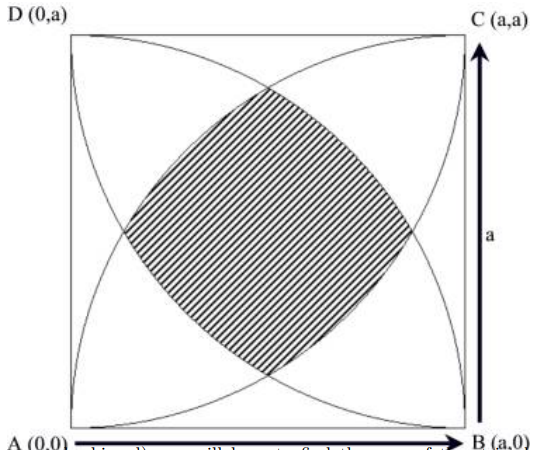
\includegraphics[width=1\textwidth]{img/area_uva}
%     \column{.6\textwidth}
%     {\bf QUIZ:}
%     \begin{itemize}
%       \item What is the area of the shaded part?
%       \item You know $a$, the radius of the 4 circles;
%     \end{itemize}\bigskip
%
%     \begin{block}{Monte Carlo Approach}
%       \begin{itemize}
%       \item Sample $N$ random points;
%       \item Calculate proportion $p$ of points in area;
%       \item Shaded area is $\frac{a^2}{p}$\bigskip
%
%       \item Mote Carlo approach is useful in several problems!
%       \end{itemize}
%     \end{block}
%   \end{columns}
% \end{frame}


% one dim measures: radius, diameter, circumference
% central angle, sector, arc
% chord: if you know the points, how to find the points if you know center and line
\begin{frame}
  \frametitle{Other circle properties}
    \begin{center}
      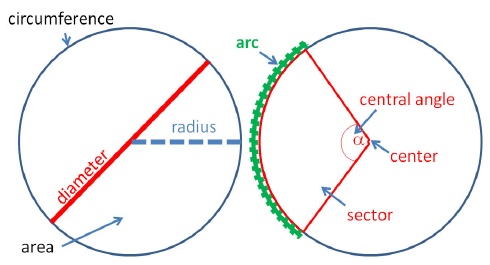
\includegraphics[width=0.5\textwidth]{../img/circle_halim0}
      \ppagenote{Circle Properties Images from Stephen Halim "Competitive Programming 3"}
    \end{center}

    \begin{itemize}
      \item {\bf radius:} $r$, {\bf diameter:} 2r, {\bf circumference:} $2\times\pi\times r$
      \item You can obtain $\pi$ from the problem, or with $\pi = 2\times \arccos(0)$
      \item Given a central angle $\alpha$:
      \begin{itemize}
        \item {\bf Arc:} $r\times\alpha$ (if in rad) or $r\times\frac{\alpha}{360}\times2\pi$ (if degrees)
        \item {\bf Sector:} $\frac{\alpha r^2}{2}$ (if in rad) or $2\pi r^2 \times \frac{\alpha}{360}$ (if degrees)
      \end{itemize}
    \end{itemize}
\end{frame}

\begin{frame}
  \frametitle{Other circle properties -- chord}
  \centering
    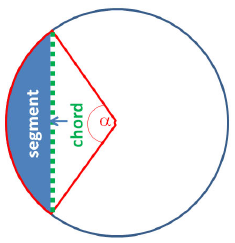
\includegraphics[width=0.25\textwidth]{../img/circle_halim1}

  \begin{itemize}
  \item {\bf chord:} Line segment with two ends in the circle's border.
  \item If you know $p_1$, $p_2$ and $c$, you can find $\alpha$ from the "angle" function;
  \item If you know $\alpha$ and $r$, you can find the size of the chord by: $|p_1p_2| = 2\times r\times\sin(\alpha/2)$
  \begin{itemize}
    \item {\bf Quiz:} If you know a line and a circle, how do you find $p_1$ and $p_2$?
  \end{itemize}
  \item If you know $p_1$, $p_2$, and $r$ (but not $\alpha$ or $c$), you can find the center of the circle using the code in the next page;
  \end{itemize}
\end{frame}

\begin{frame}[fragile]{Circle Center from points and radius}
  You have two points $p_1, p_2$ that form a chord in a circle, and the radius of that circle. How do you find the center?

  {\smaller
\begin{exampleblock}{}
\begin{verbatim}
bool circle2PtsRad(point p1, point p2, double r, point &c) {
  double d2 = (p1.x - p2.x) * (p1.x - p2.x) +
              (p1.y - p2.y) * (p1.y - p2.y);
  double det = r * r / d2 - 0.25;

  if (det < 0.0) return false; // Can't make circle

  double h = sqrt(det);
  c.x = (p1.x + p2.x) * 0.5 + (p1.y - p2.y) * h;
  c.y = (p1.y + p2.y) * 0.5 + (p2.x - p1.x) * h;
  return true;
}
// to get the other center, reverse p1 and p2
\end{verbatim}
\end{exampleblock}
  }
\end{frame}

\subsection{Triangles}

\begin{frame}
  \frametitle{Triangle Problem Example: Soya milk}
  \begin{block}{}
    \begin{itemize}
    \item {\bf Input}:\\
      The dimensions of a Milk box, and its inclination: $l, w, h, \theta$
    \item {\bf Output}:\\
      The amount of milk left in the box.
    \end{itemize}
  \end{block}

  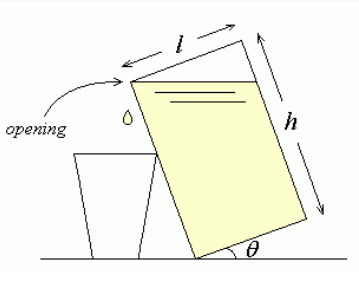
\includegraphics[width=0.4\textwidth]{img/milk_uva}
\end{frame}

\begin{frame}[t]
  \frametitle{Triangle/Circle Problem Example: Bounding Box}
  \begin{block}{}
    \begin{itemize}
      \item {\bf Input}: Three points that are the vertices of a {\bf regular polygon}, and number $n$ of sides in the polygon;\medskip
      \item {\bf Output}: Area of smallest {\bf axis aligned} rectangle that bounds this polygon.\medskip
    \end{itemize}
  \end{block}
\end{frame}

\begin{frame}
  \frametitle{Triangle Basic Facts}

    \begin{itemize}
    \item {\bf Triangle Inequality}: If $a,b,c$ are sides of a triangle, then $a+b > c; a+c > b; b+c > a$;\bigskip
    \item {\bf Perimeter, Semiperimeter}: $p = a+b+c$, $s = p/2$\bigskip
    \item {\bf Area}: $A = \frac{bh_b}{2}$\bigskip
    \item {\bf Area (Heron's formula)}: $A = \sqrt{s(s-a)(s-b)(s-c)}$\bigskip
    \item {\bf Triangulation}: Any 2D polygon can be decomposed into triangles;
  \end{itemize}
\end{frame}

\subsection{incircle}
\begin{frame}[fragile]{Incircle of a Triangle}
    \begin{columns}
      \column{0.15\textwidth}
      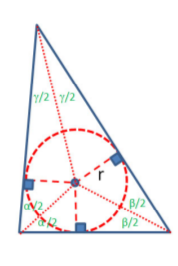
\includegraphics[width=1\textwidth]{../img/incircle_halim}
      \column{0.85\textwidth}
      \begin{itemize}
        \item An {\bf Inscribed Circle (incircle)} is the largest circle that fits inside a triangle;
        \item The radius of the incircle is: $r = A / s$
        \item The center of the circle can be found by the intersection of two {\bf angle bisectors}.
      \end{itemize}
      \end{columns}

    \begin{exampleblock}{Radius of the Incircle: $r = \text{area}/s$}
      {\smaller
\begin{verbatim}
double rInCircle(double ab, double bc, double ca) {
  return area(ab, bc, ca) / (0.5 * perimeter(ab, bc, ca)); }

double rInCircle(point a, point b, point c) {
  return rInCircle(dist(a, b), dist(b, c), dist(c, a)); }
\end{verbatim}}

    \end{exampleblock}
\end{frame}

\begin{frame}[fragile]
  \frametitle{Finding the center of the Incircle of a triangle}
  {\smaller
    \begin{exampleblock}{}
\begin{verbatim}
int inCircle(point p1, point p2, point p3, point &ctr, double &r) {
  r = rInCircle(p1, p2, p3);
  if (fabs(r) < EPS) return 0;            // Test colinear points !!!
  line l1, l2;    // we calculate the intersect of two angle bisectors

  double ratio; point p;
  ratio = dist(p1, p2) / dist(p1, p3);
  p = translate(p2, scale(toVec(p2, p3), ratio / (1 + ratio)));
  pointsToLine(p1, p, l1);                // bisector 1

  ratio = dist(p2, p1) / dist(p2, p3);
  p = translate(p1, scale(toVec(p1, p3), ratio / (1 + ratio)));
  pointsToLine(p2, p, l2);                // bisector 2

  areIntersect(l1, l2, ctr);              // find center (ctr)
  return 1;
}
\end{verbatim}
    \end{exampleblock}
    }
\end{frame}

\begin{frame}
  \frametitle{Circumcircle of a Triangle}
  \begin{columns}
    \column{0.3\textwidth}
    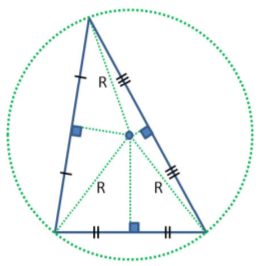
\includegraphics[width=1\textwidth]{../img/circumcircle_halim}
    \column{0.7\textwidth}
    \begin{itemize}
      \item The radius of the circumcircle in a triangle with sides $a,b,c$ and area A is $R = \frac{abc}{4A}$;
      \item The radius $R$ is also related to the {\bf Law of Sines}:
      \begin{equation*}
        \frac{a}{\sin{\alpha}} = \frac{b}{\sin{\beta}} = \frac{c}{\sin{\gamma}} = 2R
      \end{equation*}
    \end{itemize}
    \end{columns}\bigskip
    \begin{itemize}
      \item To find the center of the circumcircle:
      \begin{itemize}
        \item Use a similar algorithm as the center of the incirle (last slide);\medskip
        \item Instead of angle bisectors, use {\bf perpendicular bisectors};
      \end{itemize}
    \end{itemize}
\end{frame}

\section{Polygons}

\begin{frame}
  \centering
  {\bf Part IV -- Polygons and Convex Hull}

\end{frame}

\begin{frame}[fragile]
  \frametitle{Polygons -- Definition and data structure}

    A polygon is a plane figure bounded by a finite sequence of line
    segments.

  \begin{exampleblock}{Polygon Representation}
    \begin{itemize}
    \item In general, we store an array of points of the segments;
    \item We want to sort the points in CW or CCW order;
    \item Add the first point at the end of the array to avoid
      special cases;
    \end{itemize}
{\smaller
\begin{verbatim}
// 6 points, entered in counter clockwise order;
vector<point> P;
P.push_back(point(1, 1)); // P0
P.push_back(point(3, 3)); // P1
P.push_back(point(9, 1)); // P2
P.push_back(point(12, 4)); // P3
P.push_back(point(9, 7)); // P4
P.push_back(point(1, 7)); // P5
P.push_back(P[0]); // important: loop back
\end{verbatim}}
\end{exampleblock}
\end{frame}

\begin{frame}[fragile]
  \frametitle{Characteristics of a Polygon}
  {\smaller
    \begin{exampleblock}{Perimeter of a Poligon -- add the distances of the segments}
\begin{verbatim}
double perimeter(const vector<point> &P) {
  double result = 0.0;
  for (int i = 0; i < (int)P.size()-1; i++)
     // remember: P[0] = P[P.size()-1]
     result += dist(P[i], P[i+1]);
  return result; }
\end{verbatim}
    \end{exampleblock}

    \begin{exampleblock}{Area of a Poligon -- half of the determinant of the XY matrix of segments}
\begin{verbatim}
double area(const vector<point> &P) {
  double result = 0.0, x1, y1, x2, y2;
  for (int i = 0; i < (int)P.size()-1; i++) {
    x1 = P[i].x; x2 = P[i+1].x;
    y1 = P[i].y; y2 = P[i+1].y;
    result += (x1 * y2 - x2 * y1); }
  return fabs(result) / 2.0; }
\end{verbatim}
    \end{exampleblock}
}
\end{frame}


\begin{frame}[fragile]
  \frametitle{Testing if a Polygon is Convex}
  \begin{itemize}
    \item A convex polygon has no "holes";
    \item For any 2 points $p_1,p_2$ inside the polygon, segment is inside polygon too.
  \end{itemize}

    {\smaller
    \begin{exampleblock}{Easier Convex Testing: Every angle turns the same way}
\begin{verbatim}
bool isConvex(const vector<point> &P) {
  // Returns true if every 3 neighb vertices turn the same way;
  int sz = (int)P.size();
  if (sz <= 3) return false; // Not a polygon

  bool isLeft = ccw(P[0], P[1], P[2]); // described earlier

  for (int i = 1; i < sz-1; i++)
    if (ccw(P[i],P[i+1],P[(i+2) == sz ? 1 : i+2]) != isLeft)
      return false;            // not same direction as isLeft.

  return true;
}
\end{verbatim}
    \end{exampleblock}
  }
\end{frame}

\begin{frame}[fragile]
  \frametitle{Polygon -- Test point inside the polygon}
    % \begin{block}{There are many ways to test if a point $P$ is in a polygon.}
    %   \begin{itemize}
    %   \item \structure{Winding Algorithm}: Sum the angles of all
    %     angles $APB$ ($A,B$) are points in the polygon. If the sum is
    %     $2\pi$. Point is in polygon.
    %   \item \structure{Ray Casting Algorithm}: Draw an segment from
    %     $P$ to infinity, and count the number of polygon edges
    %     crossed. Odds: Inside. Even: Outside.
    %   \end{itemize}
    % \end{block}

  We can use the same idea to test if a point is inside the polygon: The direction of the point in relation to every edge should be the same.

    {\smaller
    \begin{exampleblock}{Winding Algorithm Code for point in polygon detection}
\begin{verbatim}
bool inPolygon(point pt, const vector<point> &P) {
  if ((int)P.size() == 0) return false;
  double sum = 0;

  for (int i = 0; i < (int)P.size()-1; i++) {
    if (ccw(pt, P[i], P[i+1]))
      sum += angle(P[i], pt, P[i+1]);       //left turn/ccw
      else sum -= angle(P[i], pt, P[i+1]);  //right turn/cw
  }

  return fabs(fabs(sum) - 2*PI) < EPS;
}
\end{verbatim}
    \end{exampleblock}
  }

  {\bf QUIZ:} What happens if the point is at an edge segment?
\end{frame}

\begin{frame}[fragile]
  \frametitle{Polygon -- Cutting}
  % TODO: Add an image explaining Polygon cutting
  {\smaller
    \begin{block}{}
      To cut $P$ along a line $AB$, we separate the points in $P$ to the
      left and right of the line.
    \end{block}

{\smaller
    \begin{exampleblock}{}
\begin{verbatim}
point lineIntersectSeg(point p, point q, point A, point B) {
  double a = B.y-A.y; double b = A.x - B.x; double c = B.x*A.y - A.x*B.y;
  double u = fabs(a*p.x + b*p.y + c); double v = fabs(a*q.x + b*q.y + c);
  return point((p.x*v + q.x*u)/(u+v), (p.y*v + q.y*u)/(u+v)); }

vector<point> cutPolygon(point a, point b, const vector<point> &Q){
  vector<point> P;
  for (int i = 0; i < (int)Q.size(); i++) {
    double left1 = cross(toVec(a, b), toVec(a, Q[i])), left2 = 0;
    if (i != (int)Q.size()-1)
      left2 = cross(toVec(a, b), toVec(a, Q[i+1]));
    if (left1 > -EPS)
      P.push_back(Q[i]);                            //Q[i] is on the left of ab
    if (left1*left2 < -EPS)                         //edge (Q[i], Q[i+1]) crosses line ab
      P.push_back(lineIntersectSeg(Q[i], Q[i+1], a, b)); }
  if (!P.empty() && !(P.back() == P.front()))
    P.push_back(P.front());                         // make P's first point = P's last point
  return P; }
\end{verbatim}
    \end{exampleblock}}
  }
\end{frame}

\begin{frame}
  \frametitle{Polygon -- Convex Hull}

  \begin{itemize}
    \item A common problem: Given a set of points $S$, what is the {\bf smallest convex polygon} that includes all points in $S$?\bigskip

    \item One way to find the Convex Hull: for each point $p \in S$, determine if the point is at the edge of the polygon (in the hull) or inside the polygon (not in the hull).\bigskip

    \item We will introduce the $O(n\log n)$ algorithm "Graham's Scan"
  \end{itemize}

    \begin{center}
      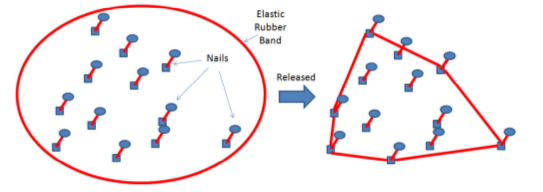
\includegraphics[width=.7\textwidth]{../img/convexhull_halim}
      \ppagenote{Convex Hull image by Steven Halim "Competitive Programming 3"}
    \end{center}
\end{frame}

\begin{frame}[fragile]
  \frametitle{Polygon -- Graham's Scan}
  \framesubtitle{Helper Functions -- sort two points based on their angle against the X axis}

{\small
\begin{exampleblock}{}
\begin{verbatim}
point pivot(0, 0);

bool angleCmp(point a, point b) {
  // special case: if collinear, choose closet to pivot;
  if (collinear(pivot, a, b)) // special case
    return dist(pivot, a) < dist(pivot, b);

  // calculate angle against the X axis:
  double d1x = a.x - pivot.x, d1y = a.y - pivot.y;
  double d2x = b.x - pivot.x, d2y = b.y - pivot.y;

  return (atan2(d1y, d1x) - atan2(d2y, d2x)) < 0;
}
\end{verbatim}
\end{exampleblock}
}
\end{frame}

\begin{frame}[fragile]
  \frametitle{Polygon -- Graham's Scan}
  \framesubtitle{Convex Hull -- Initializing the algorithm}

  {\small
    \begin{exampleblock}{}
\begin{verbatim}
vector<point> CH(vector<point> P) {
  int i, j, n = (int)P.size();
  // Special Case: Polygon with 3 points
  if (n <= 3) {
    if (!(P[0]==P[n-1])) P.push_back(P[0]);
    return P; }

  // Find Initial Point: Low Y then Right X
  int P0 = 0;
  for (i = 1; i < n; i++)
    if (P[i].y < P[P0].y ||
        (P[i].y == P[P0].y && P[i].x > P[P0].x))
      P0 = i;
  point temp = P[0]; P[0] = P[P0]; P[P0] = temp;
\end{verbatim}
\end{exampleblock}}
\end{frame}

\begin{frame}[fragile]
  \frametitle{Polygon -- Graham's Scan}
  \framesubtitle{Convex Hull -- More initialization}
  {\small
    \begin{exampleblock}{}

\begin{verbatim}

  // second, sort points by angle with pivot P0
  pivot = P[0];
  sort(++P.begin(), P.end(), angleCmp);

  // S holds the Convex Hull
  // We initialize it with first three points
  vector<point> S;
  S.push_back(P[n-1]);
  S.push_back(P[0]);
  S.push_back(P[1]);

  // We start on the third point
  i = 2;
\end{verbatim}

    \end{exampleblock}
  }
\end{frame}

\begin{frame}[fragile]
  \frametitle{Polygon -- Graham's Scan}
  \framesubtitle{Convex Hull -- Main Loop}

Now that we selected a pivot and sorted the points, we test every three points (following the sort) if they are in the convex hull.

  {\small
    \begin{exampleblock}{}
\begin{verbatim}
  while (i < n) {
    j = (int) S.size() - 1;
    // If the next point is left of CH, keep it.
    // Else, pop the last CH point and try again.

    if (ccw(S[j-1], S[j], P[i]))
      S.push_back(P[i++]);
    else
      S.pop_back();
    }
  return S;
}                 // End Graham's Scan CH
\end{verbatim}
\end{exampleblock}}
\end{frame}
%% TODO: Add polygon problem example

\section{Conclusion}

\begin{frame}
  \frametitle{Lecture Summary}

  Graph Algorithms for Path Finding and Maximum Flow:\bigskip

  \begin{itemize}
    \item Single Source Shortest Path:
    \begin{itemize}
      \item In an unweighted graph, use BFS;
      \item For a weighted graph, use Dijkstra;
      \item If the graph has negative loops, Bellman-ford will terminate;
    \end{itemize}\medskip
    \item All Pairs Shortest path:
    \begin{itemize}
      \item Floyd-Warshall is very easy to program, but costs $O(V^3)$;
      \item You could also just repeat Dijkstra $V$ times;
    \end{itemize}\medskip
    \item Maximum Flow:
    \begin{itemize}
      \item The Ford-Fergusson Method describes how to find the maximum Flow;
      \item Edmond-Karp implements FF using BFS on the residual graph to find minimum paths;
    \end{itemize}
  \end{itemize}\bigskip

  The most important skill to learn for graph problems is {\bf how to transform the problem graph}.
\end{frame}


% \subsection{Problem Discussion}
%
% \begin{frame}
%   \frametitle{This Week's Problems}
%   \begin{itemize}
%   \item Wormholes;
%   \item Meeting Professor Miguel;
%   \item Full Tank?;
%   \item Degrees of Separation;
%   \item Avoiding your Boss;
%   \item Software Allocation;
%   \item Sabotage;
%   \item Gopher II;
%   \end{itemize}
% \end{frame}
%
% \begin{frame}
%   \frametitle{Problem Hints}
%   \begin{block}{Wormholes}
%     \begin{itemize}
%     \item {\bf Problem goal:} Find a negative weight loop in the graph
%     \item {\bf Hint:} Just follow the suggestions from the class
%     \end{itemize}
%   \end{block}
%
%   \begin{exampleblock}{Meeting Professor Miguel}
%     \begin{itemize}
%     \item {\bf Problem goal:} Find the shortest path from the student to the professor.
%     \item {\bf Trick:} Some edges only the student can walk, some
%       edges only the professor can walk;
%     \item {\bf Hint 1:} There are really two graphs: One for the student, one for the
%       professor;
%     \item {\bf Hint 2:} The graphs are really small;
%     \end{itemize}
%   \end{exampleblock}
% \end{frame}
%
% \begin{frame}
%   \frametitle{Problem Hints}
%   \begin{block}{Full Tank?}
%     \begin{itemize}
%     \item Discussed in class;
%     \item Good practice on modifying graphs to solve problems;
%     \end{itemize}
%   \end{block}
%   \begin{exampleblock}{Degrees of Separation}
%     \begin{itemize}
%     \item {\bf Problem Outline:} Given a network of relationship, define the "Degree of Separation" of the network. "Degree of separation" is the {\bf largest shortest path} in the network.\bigskip
%
%     \item {\bf Hint 1:} Don't forget the special case of a disconnected Graph;
%     \item {\bf Hint 2:} The "largest shortest path" of a graph is also known as the {\bf diameter}, and it is an important property of graphs;
%     \end{itemize}
%   \end{exampleblock}
% \end{frame}
%
% \begin{frame}
%   \frametitle{Problem Hints}
%   \begin{block}{Avoiding Your Boss}
%     \begin{itemize}
%     \item {\bf Problem Goal:} You are going from your house to the market. Your boss is going from her house to the office. Can you find a path that does not meet your boss' path?\bigskip
%
%     \item {\bf Hint:} How do you modify the graph so that you can avoid your boss?
%     \end{itemize}
%   \end{block}
%
%   \begin{exampleblock}{Software Allocation}
%     \begin{itemize}
%     \item Discussed in Class;
%     \item Use this problem to practice "Max Flow";
%     \end{itemize}
%   \end{exampleblock}
% \end{frame}
%
% \begin{frame}
%   \frametitle{Problem Hints}
%   \begin{block}{Sabotage}
%     \begin{itemize}
%     \item {\bf Problem Goal:} Find the cost of minimum cut;
%     \item Discussed in class, use Max Flow to find the minimum cut set;
%     \end{itemize}
%   \end{block}
%
%   \begin{exampleblock}{Gopher II}
%     {\bf Problem Outline:}
%     \begin{itemize}
%     \item You receive the position of $N$ gophers and $M$ gopher holes.
%     \item Each hole can save 1 Gopher, Gophers run at speed $v$.
%     \item Hawks will eat the Gophers after $t$ seconds;
%     \item How many gophers are saved? How many are eatern?
%     \end{itemize}
%     {\bf Hints}:
%     \begin{itemize}
%       \item Think of an {\bf Allocation} of gophers to holes;
%       \item Graph is implicit: How do you define the edges?
%     \end{itemize}
%   \end{exampleblock}
% \end{frame}


%%%%%%%%%%%%%%%%%%%%%%%%%%%%%%%%%%%%%%%%%%%%%%%%%%%%
\section{Backmatter}
\begin{frame}{About these Slides}
  These slides were made by Claus Aranha, 2020. You are welcome to copy, re-use and modify this material.
  \bigskip

  Individual images in some slides might have been made by other
  authors. Please see the references in each slide for those cases.
\end{frame}

\begin{frame}[allowframebreaks]{Image Credits}
  \printnotes
\end{frame}

\end{CJK}
\end{document}
